\section{ZakLineObject}\label{zakLineObject}

Accepts NoteProcessors: no

Zak Line Object

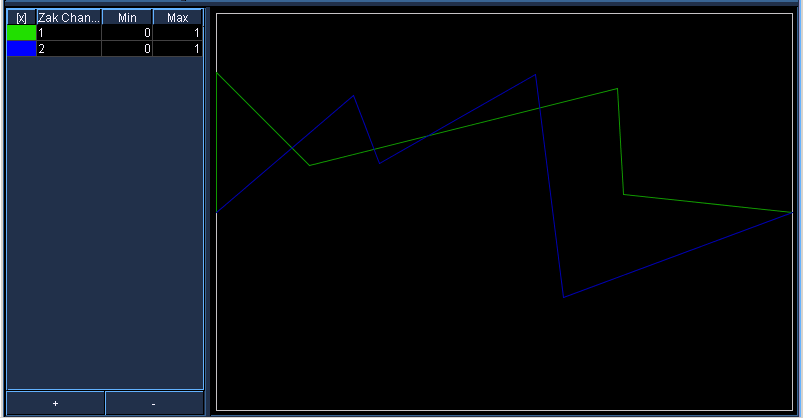
\includegraphics{images/zakLineObject.png}

Add and graphically edit zak k-rate signals.

Use the bottom + and - buttons to add/remove lines.

Use the left panel to select a line by clicking on the row describing
the line you wish to edit; you'll know which one is select by the edit
points showing up in the right panel showing the line. To edit the color
of the line, double click in the left panel on the color box to the left
of the "Zak Channel" column. A color selection dialog will appear for
the user to choose their desired color.

Enter the zak channel that you whish the signal to be written to under
the "Zak Channel" column. The "min" and "max" columns define the min and
max values of the graph that the line is drawn in to the right. However,
the min and max values can be different on a per-line basis.

When editing the line in the right panel, left clicking adds a point at
the current cursor position. Right-clicking will delete a point when a
point is under the cursor (you can easilly tell this because the a point
will change to red when the cursor is hovering over it). You can move a
point by left-clicking and dragging.
